\documentclass{report}
\usepackage{graphicx}
\usepackage{float}
\usepackage{fullpage}
\usepackage{array}
\usepackage{pdflscape}
\usepackage{multirow}
%\usepackage[T1]{fontenc}
%\usepackage{lscape}
%\usepackage[parfill]{parskip}

\setlength{\extrarowheight}{4pt}

\graphicspath{{./images/}}

\floatstyle{boxed}
\restylefloat{figure}

\begin{document}
\begin{titlepage}
\begin{center}
\vfill
\hfill
\\[2cm]
\textsc{\LARGE University Of Waterloo}
\\[1cm]
\textsc{\LARGE ECE 355}
\\[2cm]

\hrule
\hfill
\\[0.5cm]
\textsc{\huge Software Requirements Specification}
\\[0.5cm]
\textsc{\huge GARTH}
\\[0.5cm]
\textsc{\huge Green, Aware, and Responsive Total Home}
\\[0.5cm]
\hrule
\hfill
\\[1cm]
\textsc{\LARGE Group 16} \\[0.4cm]

\begin{minipage}{0.4\textwidth}
\begin{flushleft} \large
Ben Ridder \\
Casey Banner \\
Zack MacLennan
\end{flushleft}
\end{minipage}
\begin{minipage}{0.4\textwidth}
\begin{flushright} \large
brridder \\
20299452 \\
20305946 
\end{flushright}
\end{minipage}


\vfill

{\large \today}
\end{center}
\end{titlepage}

\tableofcontents
\listoffigures
\listoftables
\chapter{Introduction} % 10% Zack
\label{ch:introduction}

\section{Executive Summary}

\section{Purpose}

\section{Scope}

\section{Assumptions}

\section{Changes to Requirements}

User model defined after implementing the access array and control matrix

\section{Design Goals}

\section{Prioritization of Functionality}

\section{Terminology and Definitions}
\begin{description}
\item[RAID]
\item[Parity disk]
\item[rsync]
\item[SHA1]
\item[SQL]
\item[FIFO]
\end{description}

%\section{References}

\chapter{Architecture} % 20% - Casey
\label{ch:architecture}

\section{Overview}

The architecture of GARTH is both a layered architecture as well as a
client/server architecture. All communications-related subsystems, such as
hardware interfacing, communications protocols, and event protocols, are
layered. Subsystems such as external interfacing, inter-process communications,
and sensor communication use a client/server model.

Layering the communications subsystems will allow for more abstraction and
easier separation, leading to an increased ease of implementation for these
systems. Separating the subsystems in layers allows for parallel work to occur
on these layers, as they can individually be developed and tested before being
integrated together. An approach similar to the OSI model was chosen, with the
physical layer at the bottom. The communication subsystem layer hierarchy is
shown in Figure~\ref{fig:communication_layers}.

\floatstyle{plain}
\restylefloat{figure}
\begin{figure}[hp]
    \centering
        \caption{Communication Layer Hierarchy}
        \scriptsize
        \setlength{\unitlength}{2.0em}
        \includegraphics{communication_layers1.mps}
        \normalsize
    \label{fig:communication_layers}
\end{figure}
\floatstyle{boxed}
\restylefloat{figure}

Using a client server model allows for work to be delegated across
subsystems. GARTH relies heavily on an event-based communications model, which
is well suited to a client/server architecture. The transport layer which
facilitates this client/server model is discussed above.

Finally, at a very high level, GARTH is based on an MVC architecture pattern.
Within GARTH, the models are events which are handled by the controllers. Sensors
and output devices are the views, which generate and display data contained within
events.

% TODO: Add high level description of MVC patterns used in GARTH.

\section{Subsystem Decomposition}

% TODO: Add sensors and controllers to subsystem decomposition diagram.

% Subsystems
% - Hardware interfacing (drivers for ZigBee)
% - Communications protocol (RPC over TCP/IP)
% - Event handling (event queue)
% - External interface (JSON RPC over HTTP)
% - Sensors
% - Each controller as its own subsystem
% - Sensor OS
% - Outputs (loudspeakers, etc)

The GARTH system is composed of several subsystems. 

The subsystem decomposition is shown in Figure~\ref{fig:subsystem_decomposition}.

\floatstyle{plain}
\restylefloat{figure}
\begin{figure}[hp]
    \centering
        \caption{Subsystem Decomposition}
        \scriptsize
        \setlength{\unitlength}{2.0em}
        \includegraphics{subsystem_decomposition1.mps}
        \normalsize
    \label{fig:subsystem_decomposition}
\end{figure}
\floatstyle{boxed}
\restylefloat{figure}

The deployment diagram is shown in Figure~\ref{fig:subsystem_deployment}.

\floatstyle{plain}
\restylefloat{figure}
\begin{figure}[hp]
  \centering
  \caption{Subsystem Deployment}
  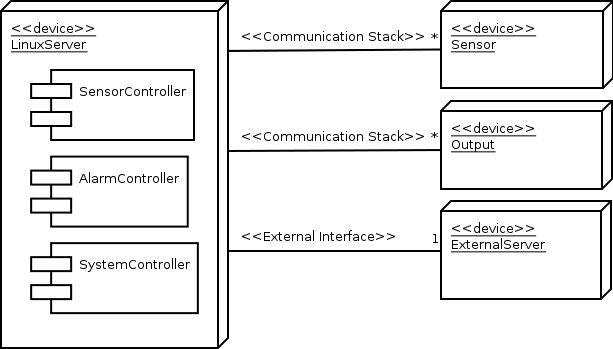
\includegraphics[scale=0.5]{deployment.png}
  \label{fig:subsystem_deployment}
\end{figure}
\floatstyle{boxed}
\restylefloat{figure}

\chapter{System Design} % 10% Zack
\label{ch:system-design}

\section{Hardware/Software Mapping}

The hardware / software mapping of the GARTH system can be viewed at a high
level by examining the subsystem decomposition at the end of Chapter 2. The
external interface and related controllers are software subsystems that are
mapped onto the Linux server. These software components interact directly with
the communications stack implemented by the server. The hardware that is mapped
to the communications stack include the sensors and the inputs and outputs of 
the system (such as control panels, alarms, speakers, etc). This hardware maps 
specifcally to the hardware interface of the communications stack which includes
all wireless and RF protocol used by the system. The communications stack also
includes the event protocol and communications protocol, which handle events
that are trigged by the hardware. Finally, the external interface to the system
is the software interface of the Linux server which will allow a user with admin
privileges to configure or manipulate the system.

\section{Data Resource Management}
%TODO mentioned proprietary software that should be fleshed out in this SDD

The two main components to GARTH's data resource management are the local
storage hardware and the remote server. The local storage component is
contained within the home and consists of a Linux server that will be stored in
a secure location. The Linux server is a desktop computer with four 2 tera byte
hard drives arranged in a modified RAID array with a parity disk for
redundancy. In this case, if a hard drive should fail the system will continue
to run as expected until a replacement hard drive gets installed. The server
will use proprietary software  to create text files that log system events as
well as store video that is captured by the cameras situated within and outside
the home.

The remote server is back-up storage that is located offsite at GARTH
headquarters. It is merely a remote backup of system logs and important video
data that should be saved for future reference. This includes any log-files or
video that was recorded by the system during a critical security violation. This
synchronization will be accomplished by using \textbf{rsync} network protocol
installed on both the local and remote server. The data that is backed up
remotely will be stored in a SQL database such that storing and querying
important data can be accomplished easily.

\section{Access Control and Security}

All access control data will be stored in the local storage database and will be
organized in an access array. The access control array will store user
information, IDs, passwords and priviliges.  This data will be encrypted using
the SHA1 hash algorithm to ensure that this data will be irrelevent to anyone
who accesses it unrightfully. This array can be accessed at any time by the
system to allow necessary access to a user. 

\begin{table}[h]
    \caption{Example of a GARTH access array}
    \label{access_array}
    \centering
    \begin{tabular}{| l | l | l | l | l | l |}
    \hline
    \textbf{Entry ID \#}&\textbf{User ID String}&\textbf{Username}&
    \textbf{Password}&\textbf{NFC ID}&\textbf{Privilege Level} \\ \hline
    1&Daryl Simpson&d\_simpson22&\$taRfi\$h&darylBB&Administrator \\ \hline
    2&Megan Simpson&msimpson&Portia&meganBold&Regular User \\ \hline
    3&Charlotte Simpson&charlotte11&Barbie11&charPod&Restricted \\
    \hline
    \end{tabular}
\end{table}

The array contains relevant information for each person who will be using the
system. The array contains a username and password for each user, in case
they need to log-in through the console's interface to change settings. Certain
settings will only be able to get changed by users with administator access.
The NFC ID field stores the device name of the NFC device the user chose to arm
or disarm the security system.

The access array is useful for determining who can gain access to the system,
however the privileges of each user will be tied separately to their respective
entry in a access control matrix. A standard access control matrix will be
employed by GARTH to solve this problem and can be seen in the table below.

\begin{table}[h]
    \caption{GARTH access control matrix}
    \label{access_control}
    \centering
    \begin{tabular}{| l | l | l | l |}
    \hline
    &\textbf{User Control}&\textbf{Data Control}&\textbf{Security Actions} \\ \hline
    \multirow{4}{*}{\textbf{Administrator}}&
    \textless\textless create\textgreater\textgreater&dumpLogs()&stopAlarms() \\
    &createUser()&searchLogs()&armSystem() \\ 
    &editUser()&viewLogs()&disarmSystem() \\
    &viewUsers()&& \\ \hline
    \multirow{2}{*}{\textbf{Regular User}}&viewUsers()&viewLogs()&armSystem() \\
    &&&disarmSystem() \\ \hline
    \multirow{2}{*}{\textbf{Restricted}}&&&armSystem() \\
    &&&disarmSystem() \\
    \hline
    \end{tabular}
\end{table}

\section{Global Software Control}

Requests are initiated by different inputs throughout the home. Most notable
would be the sensor network that generate event requests depending on the
system's armed state. For example, a window that gets opened while the security
system is armed would trigger an alarm event. Minor events are processed in a
sequential order using a very basic FIFO protocol (no concurrency). However,
events of a critical nature such as a home break-in while the system is armed
will suspend running events and get processed immediately. If more than one
critical event occurs at once, they are queued and handled sequentially while
any current suspended minor events remain suspended. This level of scheduling
will be achieved by using interrupt handling routines for the sensors that 
correspond to these events and using global priority queues.Critical events will
be designed such that they are handled quickly and efficiently in order to avoid
circumstances where critical events remained queued for long periods of time.

\section{Boundary Conditions}

A system administrator is capable of issuing requests for a server reboot, 
shutdown, or start-up if the server is powered down. The entire system relies 
on the power status of the server, and as such the user can issue these commands
from the server itself (by using its interface) or from any other control interface
in the home.

When the administrator starts the server, the controllers and sensors get
initialized in parallel. Each controller has its own separate initialization
method which starts each process in its reset state. Its own initialization
procedure takes over from here assuming initial conditions of all of its
parameters. These initalization patterns are included in the use case diagram
below as the configuration procedures that extends the initialization procedures
of each controller. The sensor initialization is a more basic procedure, as the
sensors become activated and the system polls their status by attempting 
communication between them and the sensor controller. If sensor communication
fails then a sensor error occurs and the system enters a minor alarm state.

When the administrator shuts down the server, a system snapshot is taken by
the controllers to save the state of all of the subsystems and sensors. This 
data is stored in the logs on the server, ready for when the system is started
up again. Once the snapshot is complete and the data has been stored, the power
down scheme begins which first shuts down the sensors, followed by the 
controller interfaces, and then finally the server.

A server reboot simply utilizes both of these patterns in order. First a system
shutdown is initiated, followed by a start-up immediately after.


\floatstyle{plain}
\restylefloat{figure}
\begin{figure}[hp]
    \centering
        \caption{Boundary Conditions Use Case Diagram}
        \scriptsize
        \setlength{\unitlength}{2.0em}
        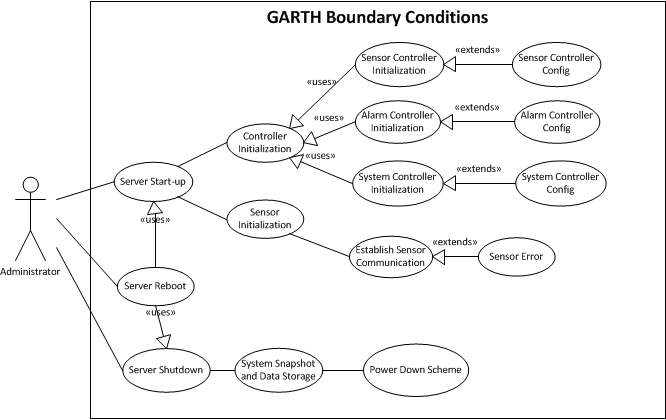
\includegraphics{boundary_conditions.png}
        \normalsize
    \label{fig:boundary_conditions}
\end{figure}
\floatstyle{boxed}
\restylefloat{figure}

\chapter{Interfaces} % 10% - Casey
\label{ch:interfaces}

\section{External System Interfaces}

A class diagram of the external interfaces that GARTH uses can be found in
Figure~\ref{fig:external_interfaces}.

\floatstyle{plain}
\restylefloat{figure}
\begin{figure}[hp]
    \centering
        \caption{External System Interfaces}
        \scriptsize
        \setlength{\unitlength}{2.0em}
        \includegraphics{external_interfaces1.mps}
        \normalsize
    \label{fig:external_interfaces}
\end{figure}
\floatstyle{boxed}
\restylefloat{figure}

All interaction with external interfaces is handled by the SystemController
component. This behaviour was chosen to reduce implementation complexity; if
only the SystemController requires access to external interfaces, then
no other Controller will have to depend on the External Interface subsystem.
This reduces both compile-time and run-time dependency.

\section{Internal Subsystem Interfaces}



\chapter{Object Design} % 30% Ben (and Casey?)
\label{ch:object-design}

% For communicationsProtocol: json-rpc.org/wiki/specification

\section{Design Patterns}
% Describe all design patterns used to reduce complexity and increase re-use in
% the system. Explain how they were applied to specifci components and the
% rationale for them.

\section{Algorithms}

\section{Packages}

\section{Object and Interface Design}

\begin{landscape} 
\floatstyle{plain}
\restylefloat{figure}
\begin{figure}[p]
    \caption{SensorController Class Diagram}
    \label{fig:sensor_controller_class_diagram}
    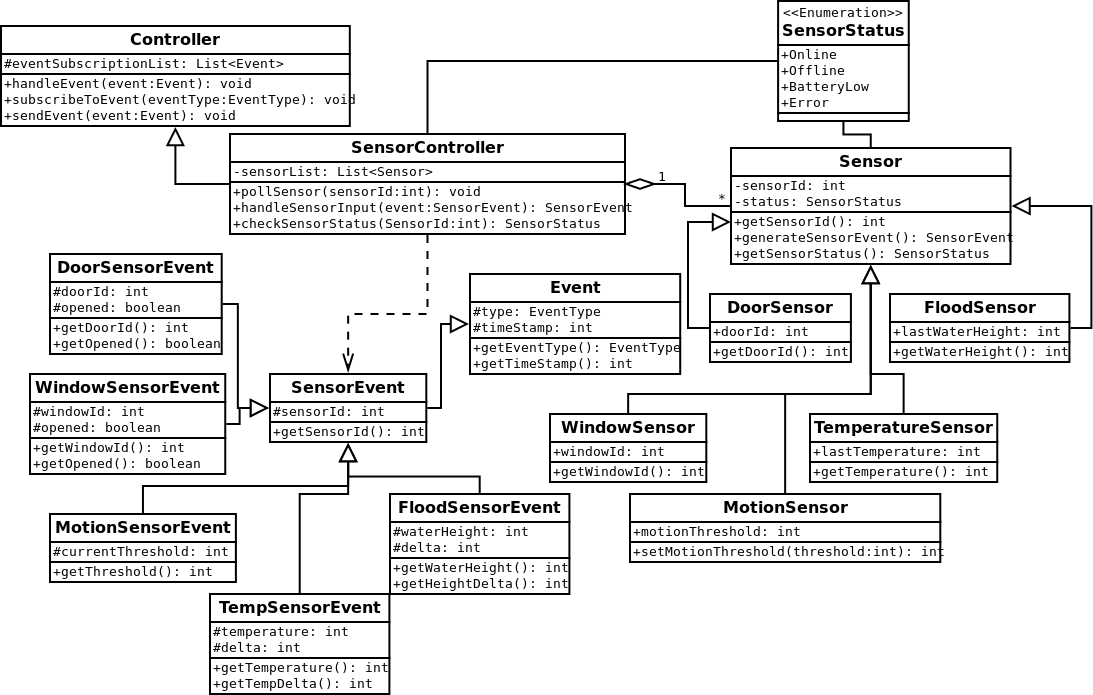
\includegraphics[scale=0.5]{sensor_controller_class_diagram.png}
\end{figure}
\end{landscape} 

\begin{landscape} 
\floatstyle{plain}
\restylefloat{figure}
\begin{figure}[p]
    \caption{SystemController Class Diagram}
    \label{fig:system_controller_class_diagram}
    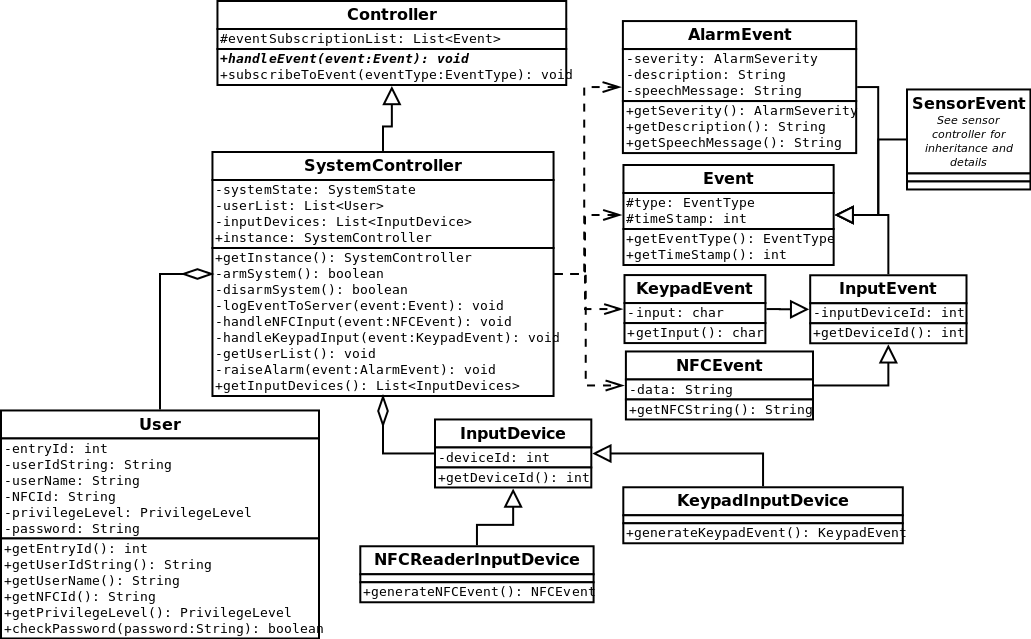
\includegraphics[scale=0.5]{system_controller_class_diagram.png}
\end{figure}
\end{landscape} 

\begin{landscape}
\floatstyle{plain}
\restylefloat{figure}
\begin{figure}[p]
    \caption{AlarmController Class Diagram}
    \label{fig:alarm_controller_class_diagram}
    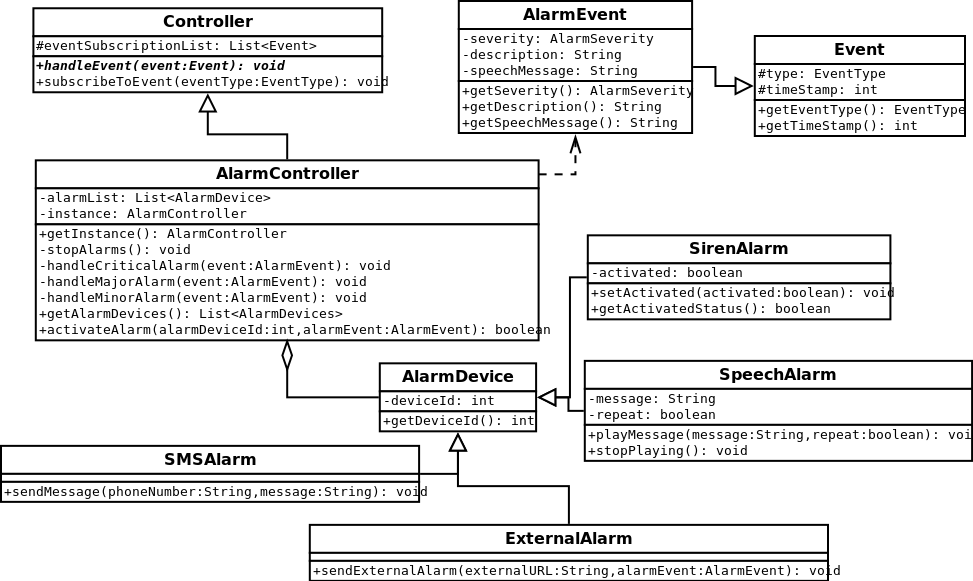
\includegraphics[scale=0.5]{alarm_controller_class_diagram.png}
\end{figure}
\end{landscape}

%\begin{landscape}
\floatstyle{plain}
\restylefloat{figure}
\begin{figure}[p]
    \caption{Communications Stack Class Diagram}
    \label{fig:communication_stack_class_diagram}
    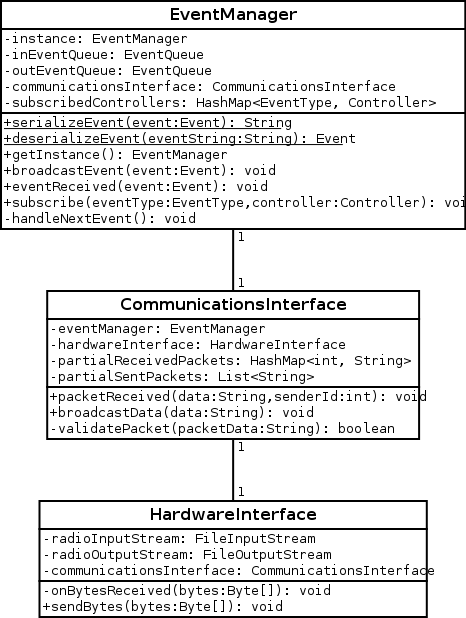
\includegraphics[scale=0.5]{communication_stack_class_diagram}
\end{figure}
%\end{landscape}

\section{Dynamic Design Model}

\chapter{Design Evaluation} % 10% Zack
\label{ch:design-evaluation}

\section{Design Trade-offs}

\section{Re-use}

\section{Optimizations}

\section{Extensibility}

\chapter{Operating Environment} % 10% Ben 
\label{ch:operating-environment}

\section{Development Platform}
%In general terms, describe the anticipated platform on which this system will
%be developed, including the implementation language, major libraries and
%network protocols utilized, and special language or OS or middleware features
%used, such as remote procedure calls, a built-in event handling model, user
%interface library, etc.

% TODO :: talk about any special language, OS, or middleware features used

Development will be done under a Linux environment as it closely matches the
intended runtime platform for the server. It also has support for all of the
required tools and libraries that are going to be used. 

Implementation language depends on the particular subsystem of the application.
The controllers will be implemented in Python for quick development and ease of 
maintenance. The sensors will need to be programmed in C for efficiency and
simplicity. Although this is not a purely Object Oriented language, using C++
would be ineffective as it results in more overhead that is to be avoided in a
real time system such as a sensor. The mobile applications will be written in
Objective-C for the iOS application and in Java for the Android version as
required by the platforms.

Several network protocols will be used. The Zigbee protocol, IEEE 802.15.4,
will be used for the hardware level communication between sensor nodes and the
base station. The protocol used between Zigbee devices will be TCP/IP. External
interfaces will use TCP/IP as well through HTTP requests for retrieving or
modifying data. 

On the iOS platform, the user interface will be constructed with the Quartz and
UIKit. These libraries provide common user interface elements such as labels,
buttons, and more. For HTTP requests, the AFNetworking library will be used as
it simplifies the handling network requests and all of the boilerplate
associated with it. On Android, the standard libraries will be used as they are
sufficient and no third party libraries exist that are provide better
functionality then the stock ones.


% Reference this: afnetworking.org/Documentation

\section{Runtime Platform}
The platform is divided into two major types of components, controllers and
sensors. Both types have different requirements for operating systems and
hardware. Middleware is required to interface between the two subsystems as well. 

The controllers will all operate on a single server as seperate processes. The
server will be a Linux based server orientated distribution such as CentOS or
Debian. The server will be housed locally within the house. The hardware needs
to be powerful, yet energy efficient and compact. No dependance on exact
hardware is required. Some recommended specifications are outlined in
Table~\ref{server_hardware}.

Each sensor will have its own independent hardware and operating system due to
the independent nature of these devices. Each will have an Atmel AVR ATMega
microcontroller for reading sensor data and communicating through the Zigbee.
The tinyOS operating system can be used to quicken development time and the
protocols for communication with the Zigbee. The tinyOS will also simplify
setting up the mesh network as several modules are provided for this.

Some middleware is required to interface the sensors and the controllers
through a Zigbee and microcontroller connected via USB to the server. A simple
hardware interface is required to allow for two-way communication between the
controllers and the sensors.

\begin{table}[h]
    \caption{Recommended Server Hardware}
    \label{server_hardware}
    \centering
    \begin{tabular}{| c | p{5cm} |}
    \hline
    Processor & AMD Athlon II X3 445 \\ \hline
    Motherboard & ASUS M5A78L-M LX PLUS AMD 760G Motherboard - Micro ATX,
    AMD 760G Chipset, 1866MHz DD3 (O.C.), SATA 3.0 Gb/s, RAID, Gigabit LAN \\
    \hline
    Case &  XION XON-810P-Red Micro ATX/ITX with 450W PSU \\ \hline
    Memory & Corsair Value Select PC10600 RAM - 2GB, DDR3, 1333Mhz \\ \hline
    Hard Drives & Western Digital Caviar Green - 2 TB x 4 \\
    \hline
    \end{tabular}
\end{table}


\section{Process Model}
%Describe whether the system is multi-threaded, runs on concurrent processes, or
%is distributed. Identify the major concurrent activities and objects (you may
%refer to the object or dynamic model), and how they will be manifested on the
%target system.

% TODO :: More
The system as a whole is distributed system, with subsystems consisting of
concurrent processes or single threaded microcontrollers. The sensor network is
one distributed subsystem that consists of many single process
microcontrollers. The controllers located on the server are concurrent
processes.

% TODO :: Refer to object/dynamic model and shit.

\section{Synchronization}
%Describe the method of coordination and synchronization between software
%tasks, such as semaphores or message queues.

% TODO :: More
Coordination and synchronization between software is done through message
queues. More specifically, the event objects are passed between interfaces and
are handled as the messages in the event queues. These event queues will
have different priority levels as some events are more critical then others in
terms of time sensitivity. 

\section{Fault Handling}
%Explain how errors will be handled. For instance, describe the use of
%exception handling in the system. Discuss how the system may recover from
%software or hardware failure.
Errors will be handled on a case by case basis as some errors will not affect
day to day operation of the system. Minor errors such as a temperature misread
or missing data from one of the passively read sensors can be ignored as long
as it is a transient event. Major errors such as a missing sensor or low
battery levels on a sensor will need to be handled. Critical errors such as a
hardware failure in the base station or server will require special care.

Minor errors can be ignored for the most part. These represent one time sensor
misreads, missing data, and other faults that do not affect any long term
operation of the system. These minor faults still need to be accounted for as
multiple occurances of this type will imply an issue with the sensor or
communication interface. When a minor error is detected, the error needs to be
logged but no further action is required.

Major errors will require system action and possibly user action to correct.
Major faults include missing sensors, low battery levels, and other issues that
will affect the short-term and long-term operation of the system. These faults
need to be accounted for and handled appropriately. In some cases, the user
will need to alerted with information on how to take the appropriate actions.
For example, if a sensor has low battery levels then the user will need to
replace or recharge the battery to ensure proper and continuous operation.

The final error criticality level is critical faults. Complete hardware or
software failures of the server can be considered critical faults. If the fault
is easily recoverable, such as a brown out causing a power flicker at the
house, then the components effected need to restart as quickly as possible to
ensure proper and consistent operation. For other faults such as hardware
failure in the base station or the server, then the user will need to take
appropriate action to fix the malfunctioning hardware.

\end{document}
